\documentclass[a4paper,12pt]{book}
\usepackage[utf8]{inputenc}
\title{}
\author{Rachel Morris}
\date{\today}

\usepackage{rachwidgets}
\usepackage{fancyhdr}
\usepackage{lastpage}
\usepackage{dirtree}
\usepackage{boxedminipage}

\setcounter{chapter}{7}
\setcounter{section}{0}
\newcommand{\laChapter}{7.1 Graph Theory\ }

\newcommand{\laClass}{CS 211\ }
\newcommand{\laSemester}{Fall 2017\ }
\newcounter{question}

\pagestyle{fancy}
\fancyhf{}
\lhead{CS 211 Exercise}
\chead{Fall 2017}
\rhead{Ch \laChapter}
\rfoot{\thepage\ of \pageref{LastPage}}
\lfoot{\scriptsize Compiled by Rachel Morris, last updated \today}

\renewcommand{\headrulewidth}{2pt}
\renewcommand{\footrulewidth}{1pt}

\begin{document}

    %\toggletrue{answerkey}
    \togglefalse{answerkey}

    \notonkey{

    %- Team Info ------------------------------------------------------%

    Please write down all people in your team. ~\\

    % table %
    \begin{tabular}{ p{6cm} p{6cm} }
        1. & 2. \\ \\
        3. & 4.
    \end{tabular}
    % table %
    ~\\

    \hrulefill

    \section{Graph Theory}

    \subsection{Terminology}

        Since we're introducing a new concept, Graph Theory,
        we need to go over the various terms so that we
        can communicate about these graphs properly.

        \begin{introNOHEAD}{}
            \begin{itemize}
                \item   \textbf{Graph:} A graph is a type of diagram that contains \textit{vertices} (aka nodes) and \textit{edges}.

                \begin{center}
                    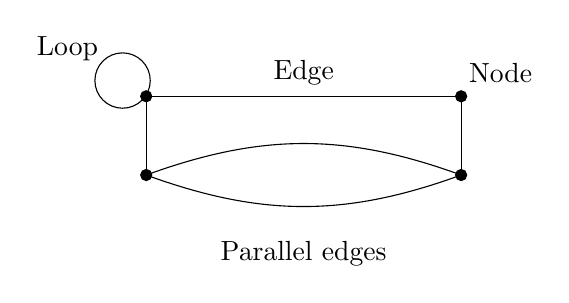
\begin{tikzpicture}
                        \filldraw (-2,0) circle (2pt);
                        \filldraw (2,0) circle (2pt);
                        \filldraw (-2,1) circle (2pt);
                        \filldraw (2,1) circle (2pt);
                        \draw (-2,0)   to[bend left=-20] (2, 0);
                        \draw (-2,0)   to[bend left=20] (2, 0);
                        \draw (2,0) -- (2,1) -- (-2,1) -- (-2, 0);

                        \node [fill=none] at (0,-1.0) {Parallel edges};
                        \node [fill=none] at (-3,1.6) {Loop};
                        \node [fill=none] at (0,1.3) {Edge};
                        \node [fill=none] at (2.5,1.3) {Node};
                        \draw (-2.3,1.2) circle (10pt);
                    \end{tikzpicture}
                \end{center}

                \item   \textbf{Node:} A vertex of the graph, drawn as a dot.
                    \begin{itemize}
                        \item   \textbf{Adjacent nodes:} Two nodes that are connected by an edge.
                        \item   \textbf{Node degree:} The amount of edges that are connected to a node.
                            Loops are counted twice.
                    \end{itemize}

                \item   \textbf{Edge:} A line that connects two nodes together.
                    \begin{itemize}
                        \item   \textbf{Parallel edges:} Two edges that have
                            the same two endpoints.
                        \item   \textbf{Loop:} An edge that begins and ends at
                            the same node, creating a loop.
                        \item   $[a, b]$ is used to indicate an edge with $a$ and $b$ as endpoints,
                            though direction can be either way.
                    \end{itemize}
            \end{itemize}
        \end{introNOHEAD}
        }{}

        \notonkey{ \newpage }{ \hrulefill }

% -------------------------------------------------------------%
% - QUESTION --------------------------------------------------%
% -------------------------------------------------------------%
\stepcounter{question}
\begin{question}{\thequestion}{6}

    Identify each item for the graph $G$ given.

    \begin{center}
        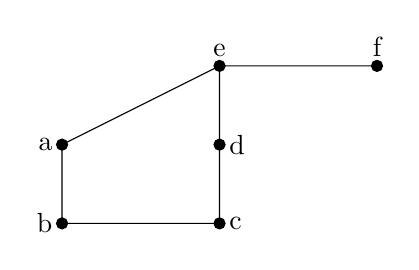
\begin{tikzpicture}
            \filldraw (0, 1) circle (2pt) node[left] {a};
            \filldraw (0, 0) circle (2pt) node[left] {b};
            \filldraw (2, 0) circle (2pt) node[right] {c};
            \filldraw (2, 1) circle (2pt) node[right] {d};
            \filldraw (2, 2) circle (2pt) node[above] {e};
            \filldraw (4, 2) circle (2pt) node[above] {f};
            \draw (4,2) -- (2,2) -- (2,1) -- (2,0) -- (0,0) -- (0,1) -- (2,2);
        \end{tikzpicture}
    \end{center}

    \begin{enumerate}
        \item[a.]   How many nodes (vertices) are there?    \solution{}{  \vspace{1cm}  }
        \item[b.]   How many edges are there?               \solution{}{  \vspace{1cm}  }
        \item[c.]   Write down the degree of each node:
            \begin{tabular}{| c | c |}
                \hline
                Vertex $v$ & $deg(v)$ \\ \hline
                $a$ & \solution{2}{} \\ \hline
                $b$ & \solution{2}{} \\ \hline
                $c$ & \solution{2}{} \\ \hline
                $d$ & \solution{2}{} \\ \hline
                $e$ & \solution{3}{} \\ \hline
                $f$ & \solution{1}{} \\ \hline
            \end{tabular}  \vspace{1cm}
        \item[d.]   The \textbf{maximum degree} of a graph is the highest $deg(v)$ value.
            What is this graph's maximum degree? \solution{3}{ \vspace{1cm} }
        \item[e.]   The \textbf{minimum degree} of a graph is the lowest $deg(v)$ value.
            What is this graph's minimum degree? \solution{1}{ \vspace{1cm} }
    \end{enumerate}

\end{question}

        \notonkey{ \newpage }{ \hrulefill }

        \notonkey{
        \begin{introNOHEAD}{\ }
            \begin{itemize}
                \item   \textbf{Walk:}   A series of alternating
                        nodes and edges, traversing between adjacent nodes.
                    \begin{itemize}
                        \item   \textbf{Closed walk:} When the beginning
                            and ending node of a walk are the same.
                        \item  \textbf{Length of a walk:} The amount
                            of edges in the walk.
                        \item   \textbf{Trivial walk:} A walk of length 0.
                        \item   \textbf{Path:} A walk with no repeated vertices.
                        \item   \textbf{Trail:} A walk with no repeated edges.
                            \begin{itemize}
                                \item   \textbf{Circuit:} A closed trail.
                                \begin{itemize}
                                    \item   \textbf{Trivial circuit:} A circuit with one vertex and no edges.
                                    \item   \textbf{Cycle:} A nontrivial circuit where the only repeated node is the first/last one.
                                \end{itemize}
                                \item   \textbf{Eulerian:} A trail or circuit where every edge is traversed.
                            \end{itemize}
                    \end{itemize}

            \end{itemize}

        \end{introNOHEAD}
        }{}

% -------------------------------------------------------------%
% - QUESTION --------------------------------------------------%
% -------------------------------------------------------------%
\stepcounter{question}
\begin{question}{\thequestion}{3}

    Answer the following questions, using the graph $H$ given.

    \begin{center}
        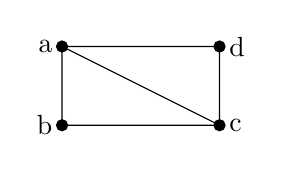
\begin{tikzpicture}
            \filldraw (0, 1) circle (2pt) node[left] {a};
            \filldraw (0, 0) circle (2pt) node[left] {b};
            \filldraw (2, 0) circle (2pt) node[right] {c};
            \filldraw (2, 1) circle (2pt) node[right] {d};
            \draw (0,1) -- (2,1) -- (2,0) -- (0,0) -- (0,1) -- (2,0);
        \end{tikzpicture}
    \end{center}

    \begin{enumerate}
        \item[a.]   Come up with several walks from $a$ to $c$. Write all steps (each node visited).
            Also label the \textbf{length} of each walk.
            \solution{ $a \to b \to c$ (2) or $a \to d \to c$ (2) or $a \to c$ (1). }{ \vspace{1cm} }
        \item[b.]   Come up with a \textbf{closed walk}, beginning and ending at $a$. You can choose to visit all nodes or not. \solution{}{ \vspace{1cm} }
        \item[c.]   Come up with a \textbf{path}, where no vertices are repeated. \solution{}{ \vspace{1cm} }
    \end{enumerate}

\end{question}

    \notonkey{ \newpage }{ \hrulefill }

% -------------------------------------------------------------%
% - QUESTION --------------------------------------------------%
% -------------------------------------------------------------%
\stepcounter{question}
\begin{question}{\thequestion}{5}

    Answer the following questions, using the graph $I$ given.

    \begin{center}
        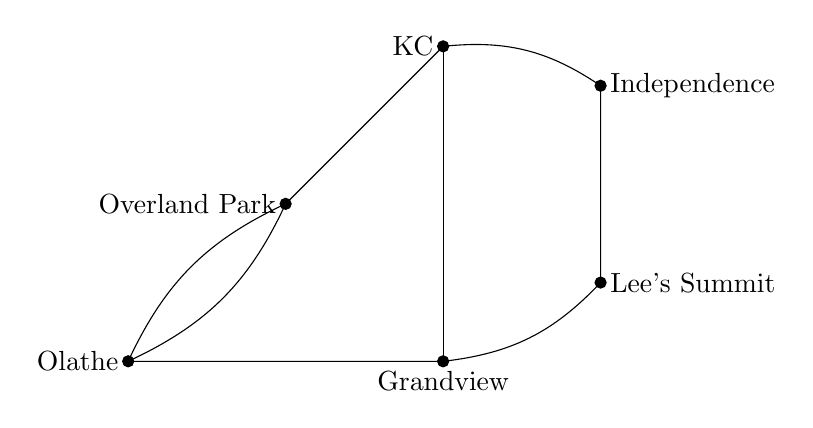
\begin{tikzpicture}
            \filldraw (0, 0) circle (2pt) node[left] {KC};
            \filldraw (-2, -2) circle (2pt) node[left] {Overland Park};
            \filldraw (-4, -4) circle (2pt) node[left] {Olathe};
            \filldraw (2,-.5) circle (2pt) node[right] {Independence};
            \filldraw (2,-3) circle (2pt) node[right] {Lee's Summit};
            \filldraw (0,-4) circle (2pt) node[below] {Grandview};

            \draw (0,0) -- (-2,-2) to[bend left=20] (-4,-4) -- (0,-4) to[bend left=-20] (2,-3) to (2,-.5) to[bend left=-20] (0,0);
            \draw (0,0) -- (0,-4);
            \draw (-4,-4) to[bend left=20] (-2,-2);
        \end{tikzpicture}
    \end{center}

    \begin{enumerate}
        \item[a.]   Come up with a \textbf{trail}, a walk with no repeated edges.
            \solution{ Example: KC $\to$ Independence $\to$ Lee's Summit }{ \vspace{1cm} }
        \item[b.]   Come up with a \textbf{circuit}, a closed trail.
            \solution{ Example: KC $\to$ Independence $\to$ Lee's Summit $\to$ Grandview $\to$ KC $\to$ Overland Park $\to$ Olathe $\to$ Grandview }{ \vspace{1cm} }
        \item[c.]   Come up with a \textbf{cycle}, a circuit where the only repeated node is the first/last one..
            \solution{ Example: KC $\to$ Independence $\to$ Lee's Summit $\to$ Grandview $\to$ KC }{ \vspace{1cm} }
        \item[d.]   Identify: Did you come up with any \textbf{Eulerian Trails}? \\ If not, create one.
            \solution{ Example: Yes, (c.) }{ \vspace{1cm} }
        \item[e.]   Identify: Are there any \textbf{parallel edges}?
            \solution{ Yes: Olathe $\to$ Overland Park }{ \vspace{1cm} }
    \end{enumerate}
\end{question}

    \notonkey{ \newpage }{ \hrulefill }

    \notonkey{
    \begin{introNOHEAD}{}
        \begin{itemize}
            \item   \textbf{Simple graph:} A graph that has no loops or parallel edges.
            \item   \textbf{Directed graph:}    The edges in the graph are given a direction, which can only be traversed in that way.
                \begin{itemize}
                    \item   Edges are denoted with parentheses $(a, b)$, showing that it goes from $a$ to $b$.
                \end{itemize}
        \end{itemize}
    \end{introNOHEAD}
    }{}

% -------------------------------------------------------------%
% - QUESTION --------------------------------------------------%
% -------------------------------------------------------------%
\stepcounter{question}
\begin{question}{\thequestion}{1}

    Draw a \textbf{Directed Graph} using the following list of edges:

    $$ (1,2), (2,1), (3,3), (4,2) $$

    (Don't confuse these for points on an $x,y$ plane that are interconnected,
    each ordered pair is its own set of information - beginning and end nodes.)

    \solution{ Multiple solutions }{}

\end{question}

    \vspace{1cm}

    \notonkey{
    \begin{introNOHEAD}{}
        \begin{itemize}
            \item   A graph is \textbf{connected} if there is a walk between any pair of distinct nodes.
            \item   A graph $H$ is a \textbf{subgraph} of a graph $G$ if all nodes and edges in $H$ are also
                nodes and edges in $G$.
            \item   A \textbf{connected component} of a graph $G$ is a connected subgraph $H$ of $G$ such
                that no other connected subgraph of $G$ containing $H$ exists.
        \end{itemize}
        \footnote{Discrete Mathematics, Ensley and Crawley}
    \end{introNOHEAD}
    }{}


% -------------------------------------------------------------%
% - QUESTION --------------------------------------------------%
% -------------------------------------------------------------%
\stepcounter{question}
\begin{question}{\thequestion}{2}

    Draw a graph that is \textbf{not connected}, and draw a \textbf{subgraph} of your graph.

    \solution{ Multiple solutions }{}

\end{question}



\end{document}
